\section{System-Layering und Modulstruktur}

\subsection{Strukturierung des Engine-Kerns}

Die Strukturierung der Engine folgt der im Prototyp-Dokument beschriebenen Unterteilung in Module und orientiert sich weitgehend an einem \textit{by-feature, by-layer}-Ansatz, wie in Abbildung~\ref{fig:engine_struktur} dargestellt.\\

\begin{figure}[!htbp]
    \setlength{\DTbaselineskip}{18pt}
    \dirtree{%
        .1 ./engine.
        .2 builder/.
        .2 common/.
        .2 core/.
        .2 ecs/.
        .2 mechanics/.
        .2 modules/.
        .2 runtime/.
        .2 tooling/.
    }
    \caption{Struktur des \texttt{engine}-Moduls von \textit{helios}.}
    \label{fig:engine_struktur}
\end{figure}

Die Unterteilung der Module gestaltet sich dabei wie folgt:

\begin{itemize}
    \itemsep0.5em
    \item \texttt{builder/}: Stellt \textit{Builder}-Klassen für Spawn-Systeme und GameObjects bereit.
    Diese basieren auf Expression Builder, Fluent Interfaces sowie einer DSL, um die Konfiguration von Fachobjekten aus einem hohen Abstraktionsgrad in einen intuitiveren Kontext zu überführen.
    \item \texttt{common/}: Enthält allgemeine Hilfsklassen, die vor allem von \texttt{mechanics} und \texttt{modules} genutzt werden, darunter spielspezifische Kontextklassen für systemübergreifende Informationen.
    \item \texttt{core/}: Stellt fundamentale Datentypen und Objekte zur Verfügung, die für den Betrieb der Engine benötigt werden, wie beispielsweise \texttt{Units}, in der das metrische System für \textit{helios} definiert ist.
    \item \texttt{ecs/}: Implementiert die Kernkomponenten der ECS-Architektur, darunter den \texttt{EntityManager}, die \texttt{GameObject}-Fassade und die \texttt{SparseSet}-Datenstruktur.
    \item \texttt{mechanics/}: Implementiert Komponenten, Systeme, Datentypen und Nachrichtenobjekte für spezifische Spielmechaniken (z.\,B. Eingabeverarbeitung, Gesundheits- und Schadenslogik sowie Punktesysteme).
    \item \texttt{modules/}: Stellt Subsysteme mit einer höheren Nähe zum Engine-Kern bereit.
    Dazu zählen Domänen wie \texttt{ai}, \texttt{physics} und \texttt{rendering}, die hierdurch auch die Infrastruktur für Gameplay liefern.
    \item \texttt{runtime/}: Beinhaltet laufzeitnahe Kernsysteme wie \texttt{messaging}, \texttt{gameloop} und \texttt{world}.
    Diese C++-Module enthalten neben Datenstrukturen auch \textit{Manager}-Klassen.
    Ihre Implementierung ist weitgehend generisch gehalten; darauf aufbauende Fachlogiken sind in \texttt{mechanics} und \texttt{modules} ausgelagert.
    \item \texttt{tooling/}: Bildet das Tooling-Layer der Engine.
    Es enthält aktuell Hilfsklassen zur Erfassung von Performance-Metriken, darunter \texttt{FrameStats}.
    Diese werden pro Frame $N$ diskret aufgezeichnet und den Systemen zur weiteren Verarbeitung in Frame $N+1$ zur Verfügung gestellt.
\end{itemize}

Eine schematische Darstellung der Architektur findet sich in Abbildung~\ref{fig:layered_engine_architecture}.

\begin{figure}[!htbp]
    \centering
    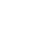
\includegraphics[width=1.0\columnwidth]{content/de/architektur/img/layered_engine_architecture}
    \caption{Logische Gliederung der Engine-Schichten in \textit{helios}. Als Orchestrator und Verwalter kapselt Runtime die Module \texttt{mechanics} und \texttt{modules}, die domänenspezifische und wiederverwendbare Klassen enthalten und auf der Runtime-Infrastruktur aufbauen. Die Laufzeitschicht nutzt Definitionen und Implementierungen aus \texttt{ecs}- und \texttt{core}. Das Modul \texttt{tooling} realisiert \textit{Cross-cutting concerns}~\cite{KLMM+97} und ist deshalb querschnittlich dargestellt.  (Quelle: eigene Darstellung)}
    \label{fig:layered_engine_architecture}
\end{figure}

\subsection{Namenskonvention für tiefere Schichten}

Innerhalb der Module nutzt \textit{helios} zur eindeutigen Identifizierung und technischen Zuordnung der Fachobjekte die folgenden Namenskonventionen zur Verortung von Implementierungen:

\begin{itemize}
    \itemsep0.5em
    \item \texttt{commands}: Steuerkommandos, die innerhalb eines Frames von Systemen und Managern generiert werden.
    Die Verarbeitung erfolgt über \texttt{CommandHandler}-Konzepte, auf die in Abschnitt~\ref{sec:runtime_messaging} näher eingegangen wird.
    \item \texttt{components}: Objekte, die fachlich unterschiedliche Zustände eines GameObjects repräsentieren.
    Als primär datenhaltende \texttt{struct}s konzipiert, können diese Objekte auch Invarianten absichern, etwa durch \textit{Clamping} von Werten.
    Sie sollten darüber hinaus jedoch kein Verhalten implementieren.\footnote{
        Im Gegensatz zu unserem Konzept, das auch eine Absicherung von Invarianten berücksichtigt, sehen andere ECS-Architekturen wie \textit{Unity DOTS} vor, dass Komponenten als reine Informationsträger fungieren: Invarianten werden dort in den Systemen abgesichert~\cite{UnityComponentConcepts}.
    }
    \item \texttt{events}: Nachrichten, die Systeme in Frame $N$ generieren und die von nachgelagerten Systemen im selben Frame oder in Frame $N+1$ verarbeitet werden können.
    Im Gegensatz zu \texttt{Commands} sind \textit{Events} als Informationsträger konzipiert.
    Sind deterministische Aktionen gefragt, sollten \texttt{Commands} verwendet werden.
    Die Unterscheidung existiert in \textit{helios} jedoch nur auf semantischer Ebene.
    \item \texttt{systems}: Logikeinheiten, die das Verhalten von GameObjects modifizieren, indem sie Komponenten aktualisieren sowie \texttt{Commands} und \texttt{Events} emittieren.
    \item \texttt{types}: Hilfstypen wie Kontextobjekte~\cite[182-204]{ACM03} zum Datentransport sowie typisierte Ids zur sicheren Identifizierung von Ressourcen zur Laufzeit.
\end{itemize}

\begin{figure}[!htbp]
    \setlength{\DTbaselineskip}{18pt}
    \dirtree{%
        .1 ./mechanics/health/.
        .2 components/.
        .3 HealthComponent.ixx.
        .2 events/.
        .3 HealthChangedEvent.ixx.
        .3 HealthDepletedEvent.ixx.
        .2 systems/.
        .3 HealthUpdateClearSystem.ixx.
        .2 types/.
        .3 HealthChangeContext.hpp.
        .3 HealthDepletedBehavior.hpp.
    }
    \caption{Veranschaulichung der Namenskonventionen in \textit{helios} anhand der \textit{health}-Spielmechanik.
    Die \texttt{HealthComponent} beinhaltet Eigenschaften wie einen skalaren HP-Wert sowie Methoden, über die Invarianten abgesichert werden.}
    \label{fig:health_struktur}
\end{figure}

Während \texttt{types}, \texttt{events} und \texttt{commands} aufgrund ihrer universellen Semantik in verschiedenen Schichten vorkommen, finden sich \texttt{systems} überwiegend in den Modulen \texttt{mechanics} und \texttt{modules}.
Ihre Rolle ist untrennbar mit dem ECS-Kern in \textit{helios} verbunden; ihre Ausführung erfolgt primär über die in \texttt{runtime} definierten Laufzeitsysteme.